\section{Моделирование диаграммообразования итеративным методом}\label{sect:iterative-modeling}

Программа для моделирования схожа с той, что использовалась 
в разделе с амплитудными и геометрическими распределениями. 
Моделирование проводилось для антенной решётки, заданной согласно методу, описанному в разделе \ref{sect:iterative-theory}.

Установим координаты исходной эквидистантной решётки

\begin{minted}[
    linenos,
    breaklines,
    frame=single,
    framesep=10pt
]{matlab}
f = 3e9; % 3 GHz text
lam = freq2wavelen(f); % длина волны
xmin = 0;xmax = 29; % количество элементов
dOk = lam/2; % межэлементное расстояние
dxOk = dOk*(xmin:1:xmax)'; % координаты элементов     
\end{minted}

Сформируем исследуемую разреженную решётку с помощью удаления 12 элементов из исходной решётки и 
добавления двух элементов на её краях. Отдельно зададим центральную эквидистантную подрешётку.

\begin{minted}[
    linenos,
    firstnumber=last,
    breaklines,
    frame=single,
    framesep=10pt
]{matlab}
dxRare = [-2*dOk; dxOk([1 3 5 9:20 26 28 30]); 33*dOk];
dxRare2 = dxOk([9:20]);   
\end{minted}

Получим распределения сигналов на заданных решётках

\begin{minted}[
    linenos,
    firstnumber=last,
    breaklines,
    frame=single,
    framesep=10pt
]{matlab}
valuesOk = distribution_former(dxOk,f,aimAngles, aimAmps); % значение сигнала на элементах исходной решётки
valuesRare = distribution_former(dxRare,f,aimAngles, aimAmps);  % значение сигнала на элементах исходной решётки
valuesRare2 = valuesOk([9:20]); % значение сигнала на центральной подрешётке
\end{minted}

Дополнительно формируются значения со спадающими амплитудными распределениями

\begin{minted}[
    linenos,
    firstnumber=last,
    breaklines,
    frame=single,
    framesep=10pt
]{matlab}
valuesRare1 = valuesRare.*([[1,1, 3, 5, 6, 6.5, 7, 7.4, 7.7,8] fliplr([1,1, 3, 5, 6, 6.5, 7, 7.4, 7.7,8])]');
valuesRare21 = valuesRare2.*([[5, 5, 5.5, 6, 6, 6.5] fliplr([5, 5, 5.5, 6, 6, 6.5])]');  
\end{minted}

Далее проводится сканирование и перемножение пространственных откликов

\begin{minted}[
    linenos,
    firstnumber=last,
    breaklines,
    frame=single,
    framesep=10pt
]{matlab}
[rstOk,theta] = aec_simulation(valuesOk, dxOk,f); % ДН эквидистантной решётки для сравнения
rstRare = aec_simulation(valuesRare, dxRare,f); % ДН разрженной решетки для сравнения
rstRare1 = aec_simulation(valuesRare1, dxRare,f);
rstRare2 = aec_simulation(valuesRare2, dxRare2,f); % ДН центарльной решётки для сравнения
rstRare21 = aec_simulation(valuesRare21, dxRare2,f);
rstRare3 = rstRare21.*rstRare; % результирующая ДН
\end{minted}

Для оценки результатов работы данного алгоритма, по методу из раздела \ref{sec:perturbations-method} был сформирован 
ещё один разреженный массив с расширяющимся к краям геометрическим распределением.

Рассмотрим результаты моделирования на Рисунке \ref{iterative-array-raw-beam-pattern}. Как видно, отклик разреженных 
решёток имеет сравнимый по ширине главный лепесток, однако ДН решётки разреженной методом 
удаления имеет даже бОльшую величину УБЛ, чем у эквидистантной, 
и при этом обе разреженные решётки имеют довольно высокие уровни дифракционных лепестков.

\begin{figure}[!ht]
    \centering
    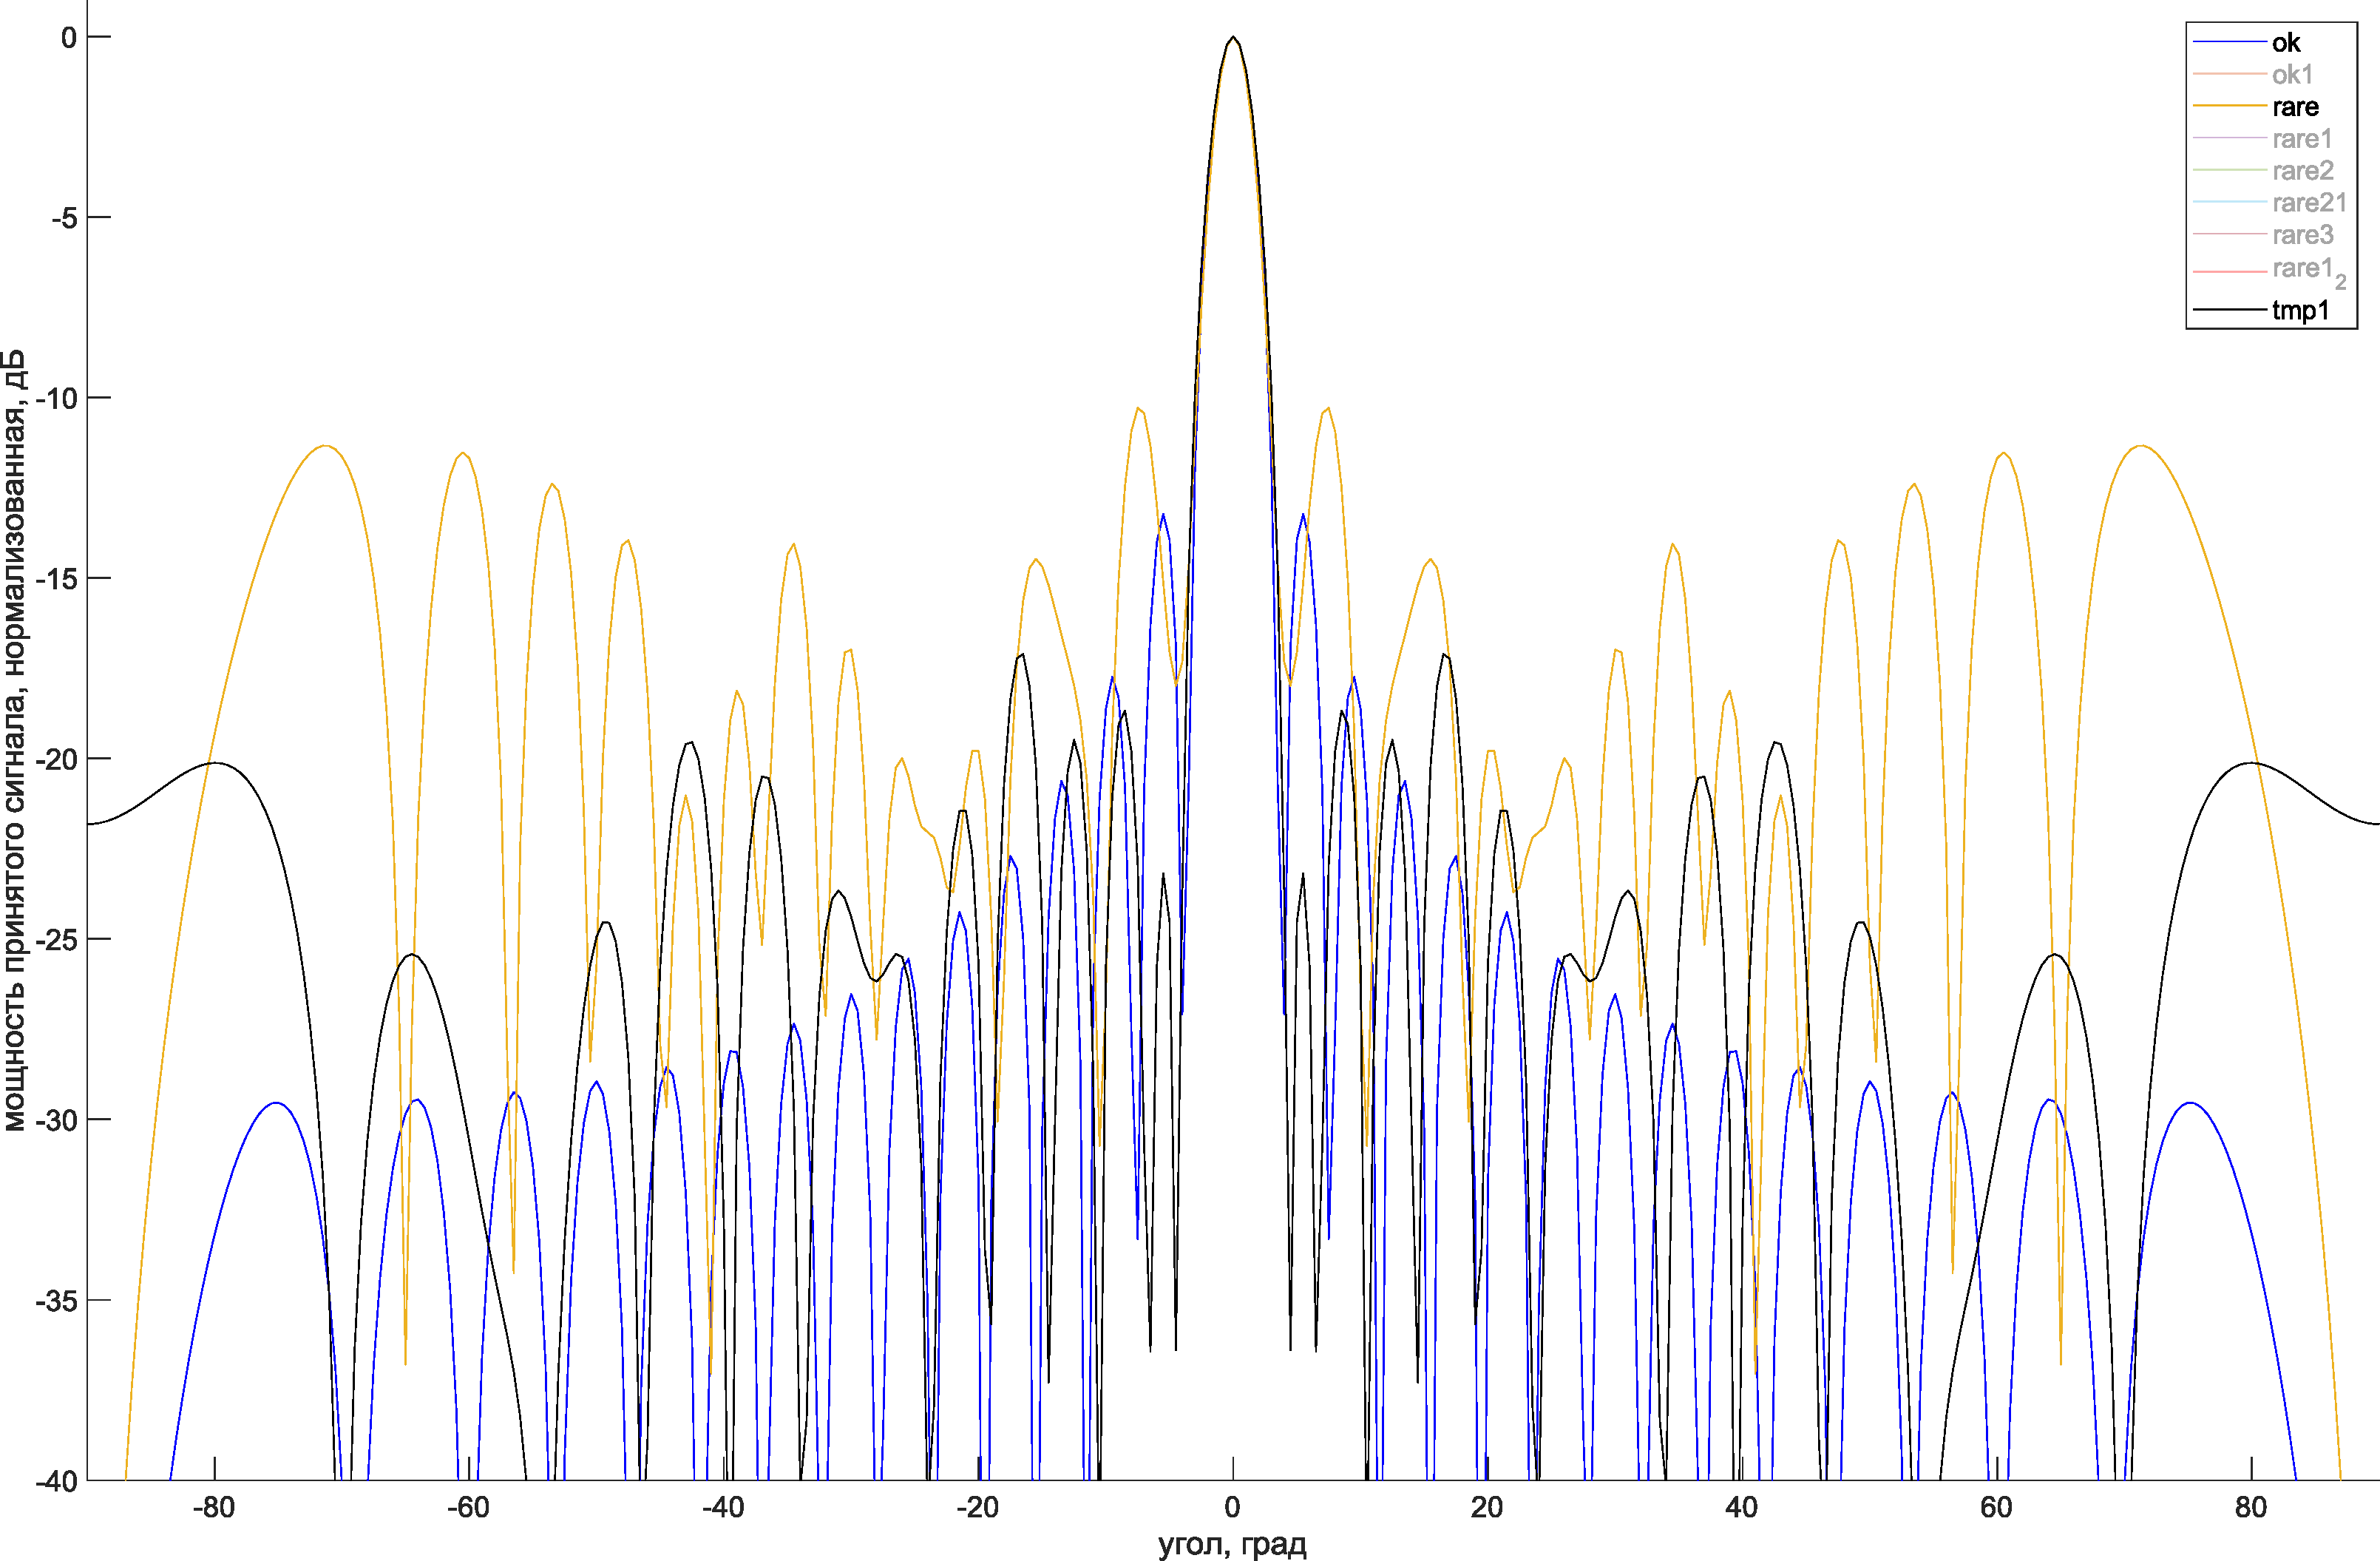
\includegraphics[width=0.8\textwidth,height=0.35\textheight,keepaspectratio]{iterative-array-raw-beam-pattern}
    \caption{Сравнение пространственных откликов от 
    (синий) эквидистантной решётки из 30 элементов
    (жёлтый) разреженной решётки из данного метода
    (чёрный) разреженной решётки с расширяющимся к краям распределением, сформированным по методике из раздела \ref{sec:perturbations-method}
    }%
    \label{fig:iterative-array-raw-beam-pattern}
\end{figure}

Сравним данные результаты с результатами полученными методом итеративной обработки данных. Результат показан на Рисунке \ref{fig:iterative-array-processed-beam-pattern}. 
Диаграмма направленности, полученная в результате применения данного метода, имеет меньший уровень боковых лепестков чем у равномерного и классического неравномерного распределений при той же ширине главного лепестка.Дифракционные лепестки также на низком уровне. 

\begin{figure}[H]
    \centering
    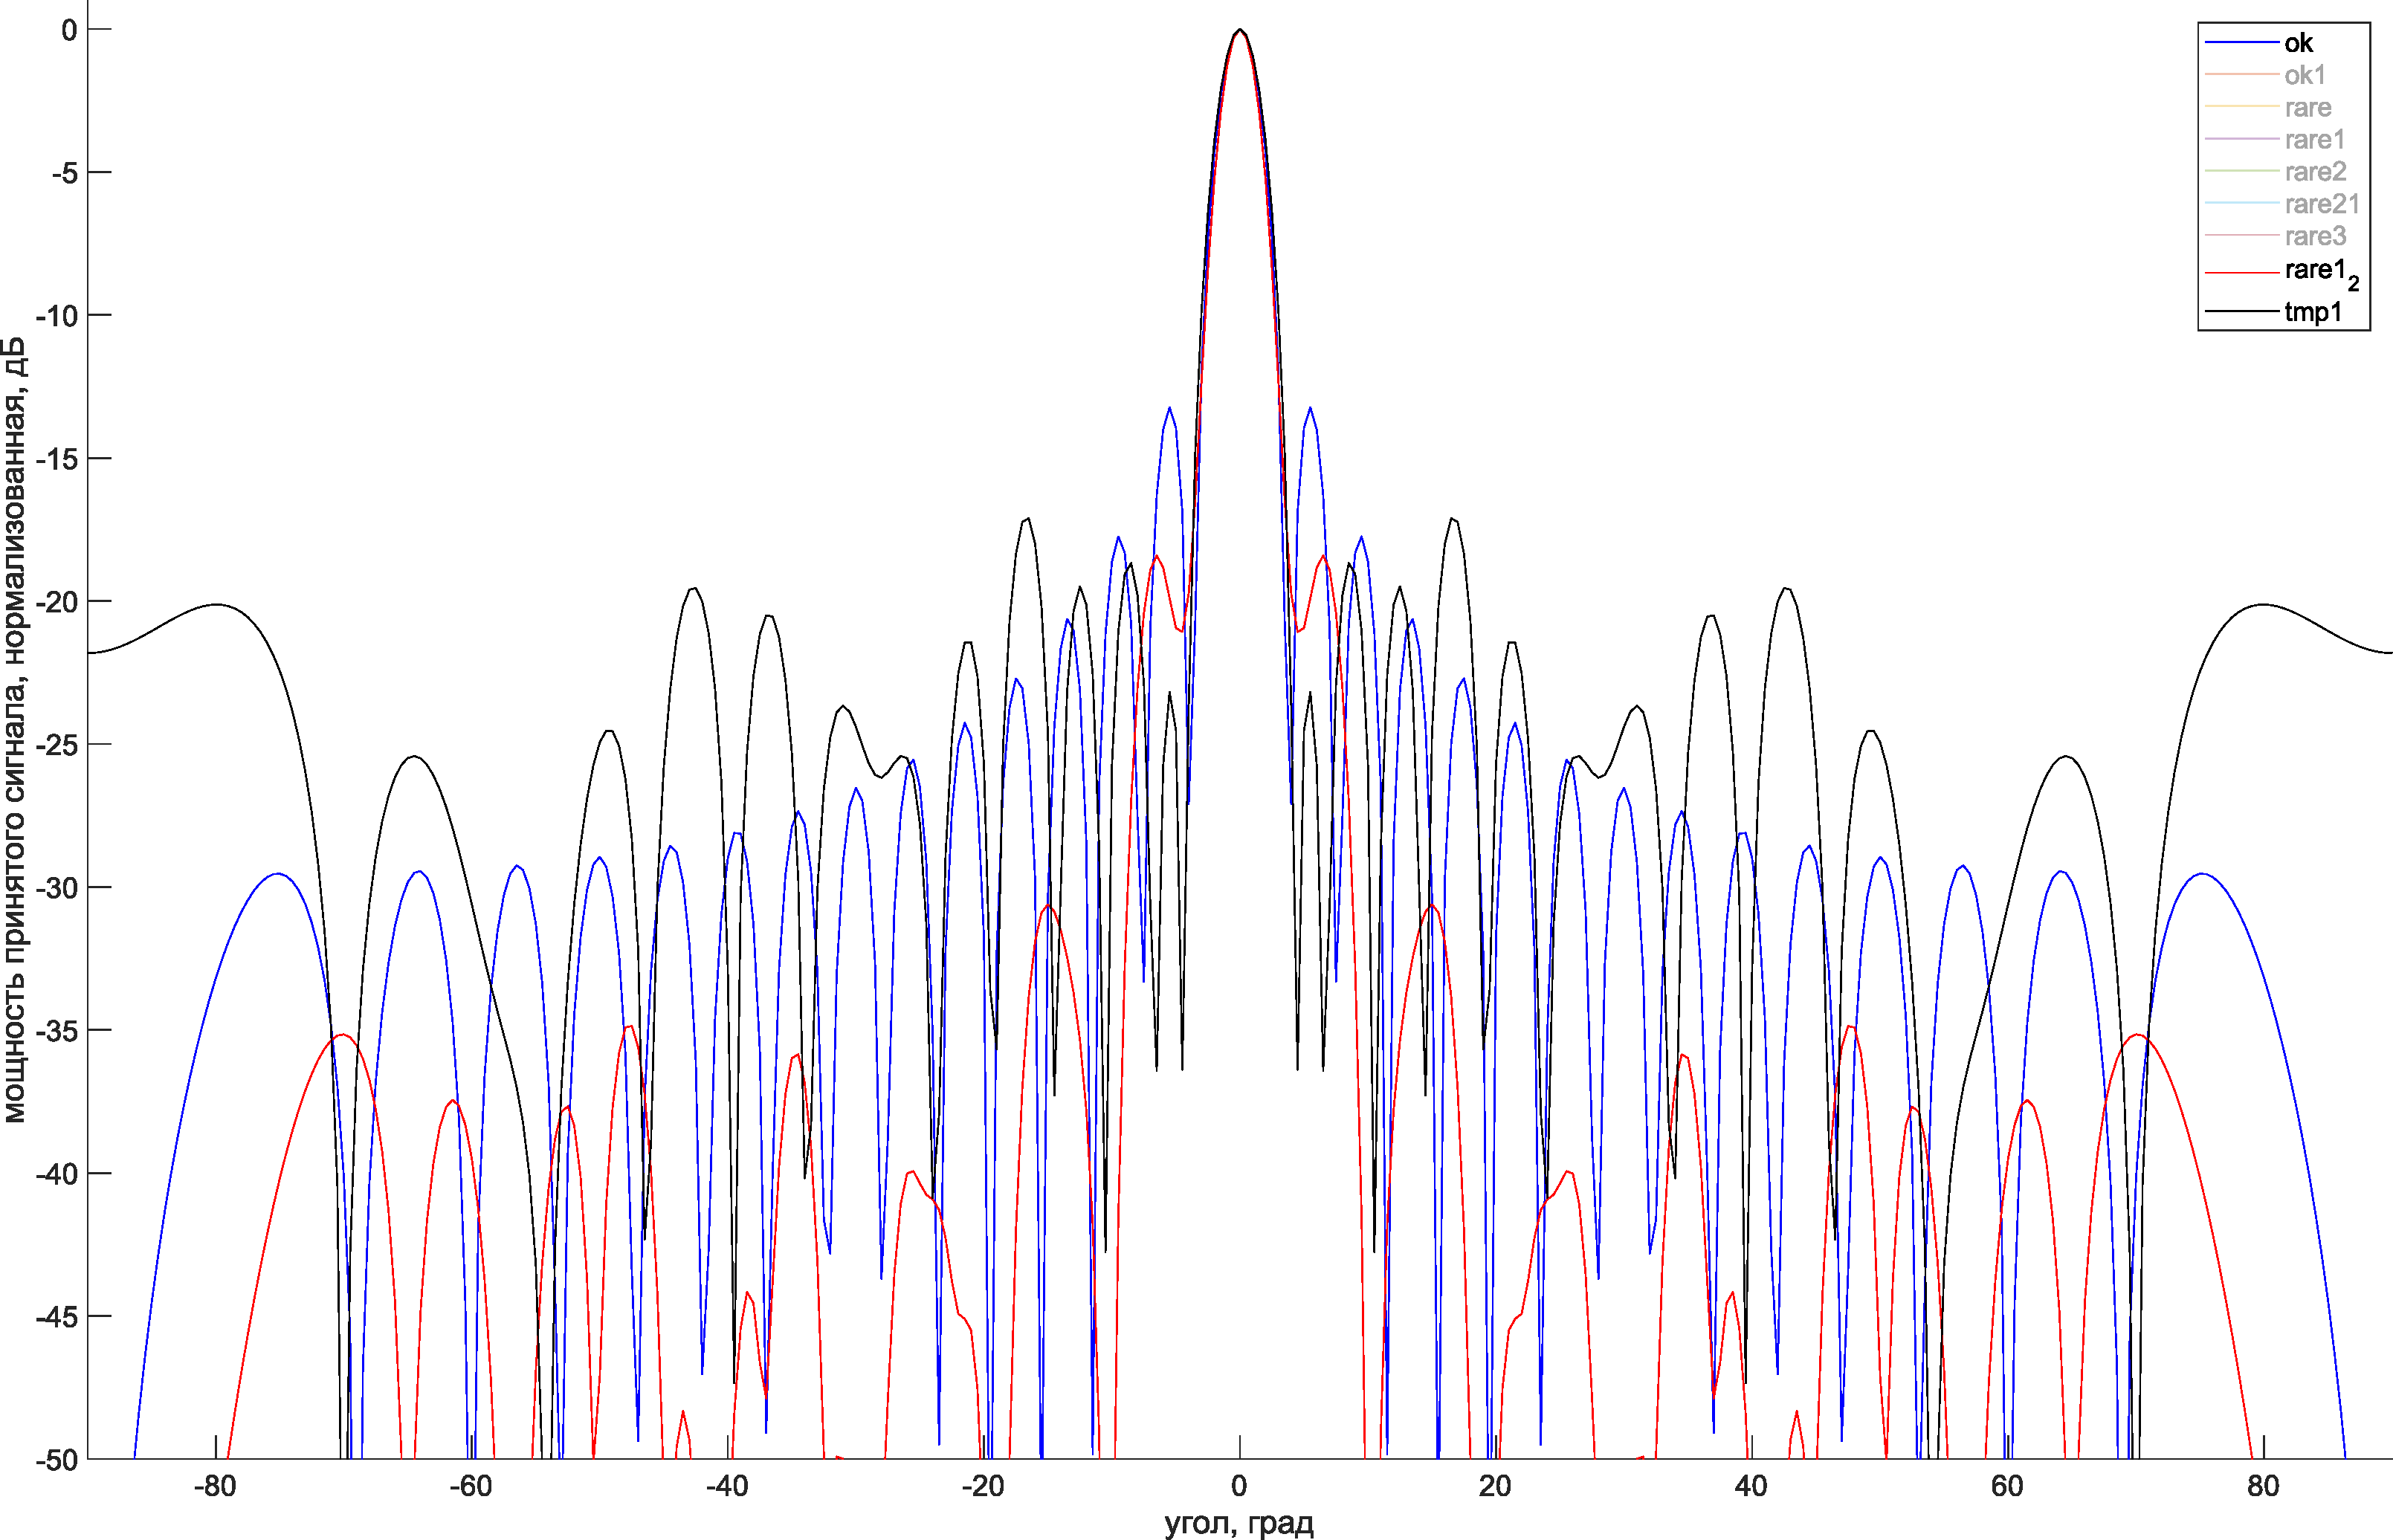
\includegraphics[width=0.8\textwidth,height=0.35\textheight,keepaspectratio]{iterative-array-processed-beam-pattern}
    \caption{Сравнение пространственных откликов от 
    (синий) эквидистантной решётки из 30 элементов
    (красный) синтезированной решётки из данного метода
    (чёрный) разреженной решётки с расширяющимся к краям распределением, сформированным по методике из раздела \ref{sec:perturbations-method}
    }%
    \label{fig:iterative-array-processed-beam-pattern}
\end{figure}

Рассмотрим также следующую демосцену: зададим 4 сигнала с разной амплитудой

\begin{minted}[
    linenos,
    breaklines,
    frame=single,
    framesep=10pt
]{matlab}
aimAngles = [0 -20 30 50];
aimAmps   = [0 -1 -4 -2];
\end{minted}

Результат показан на Рисунке~\ref{fig:iterative-array-demo}

\begin{figure}[!ht]
    \centering
    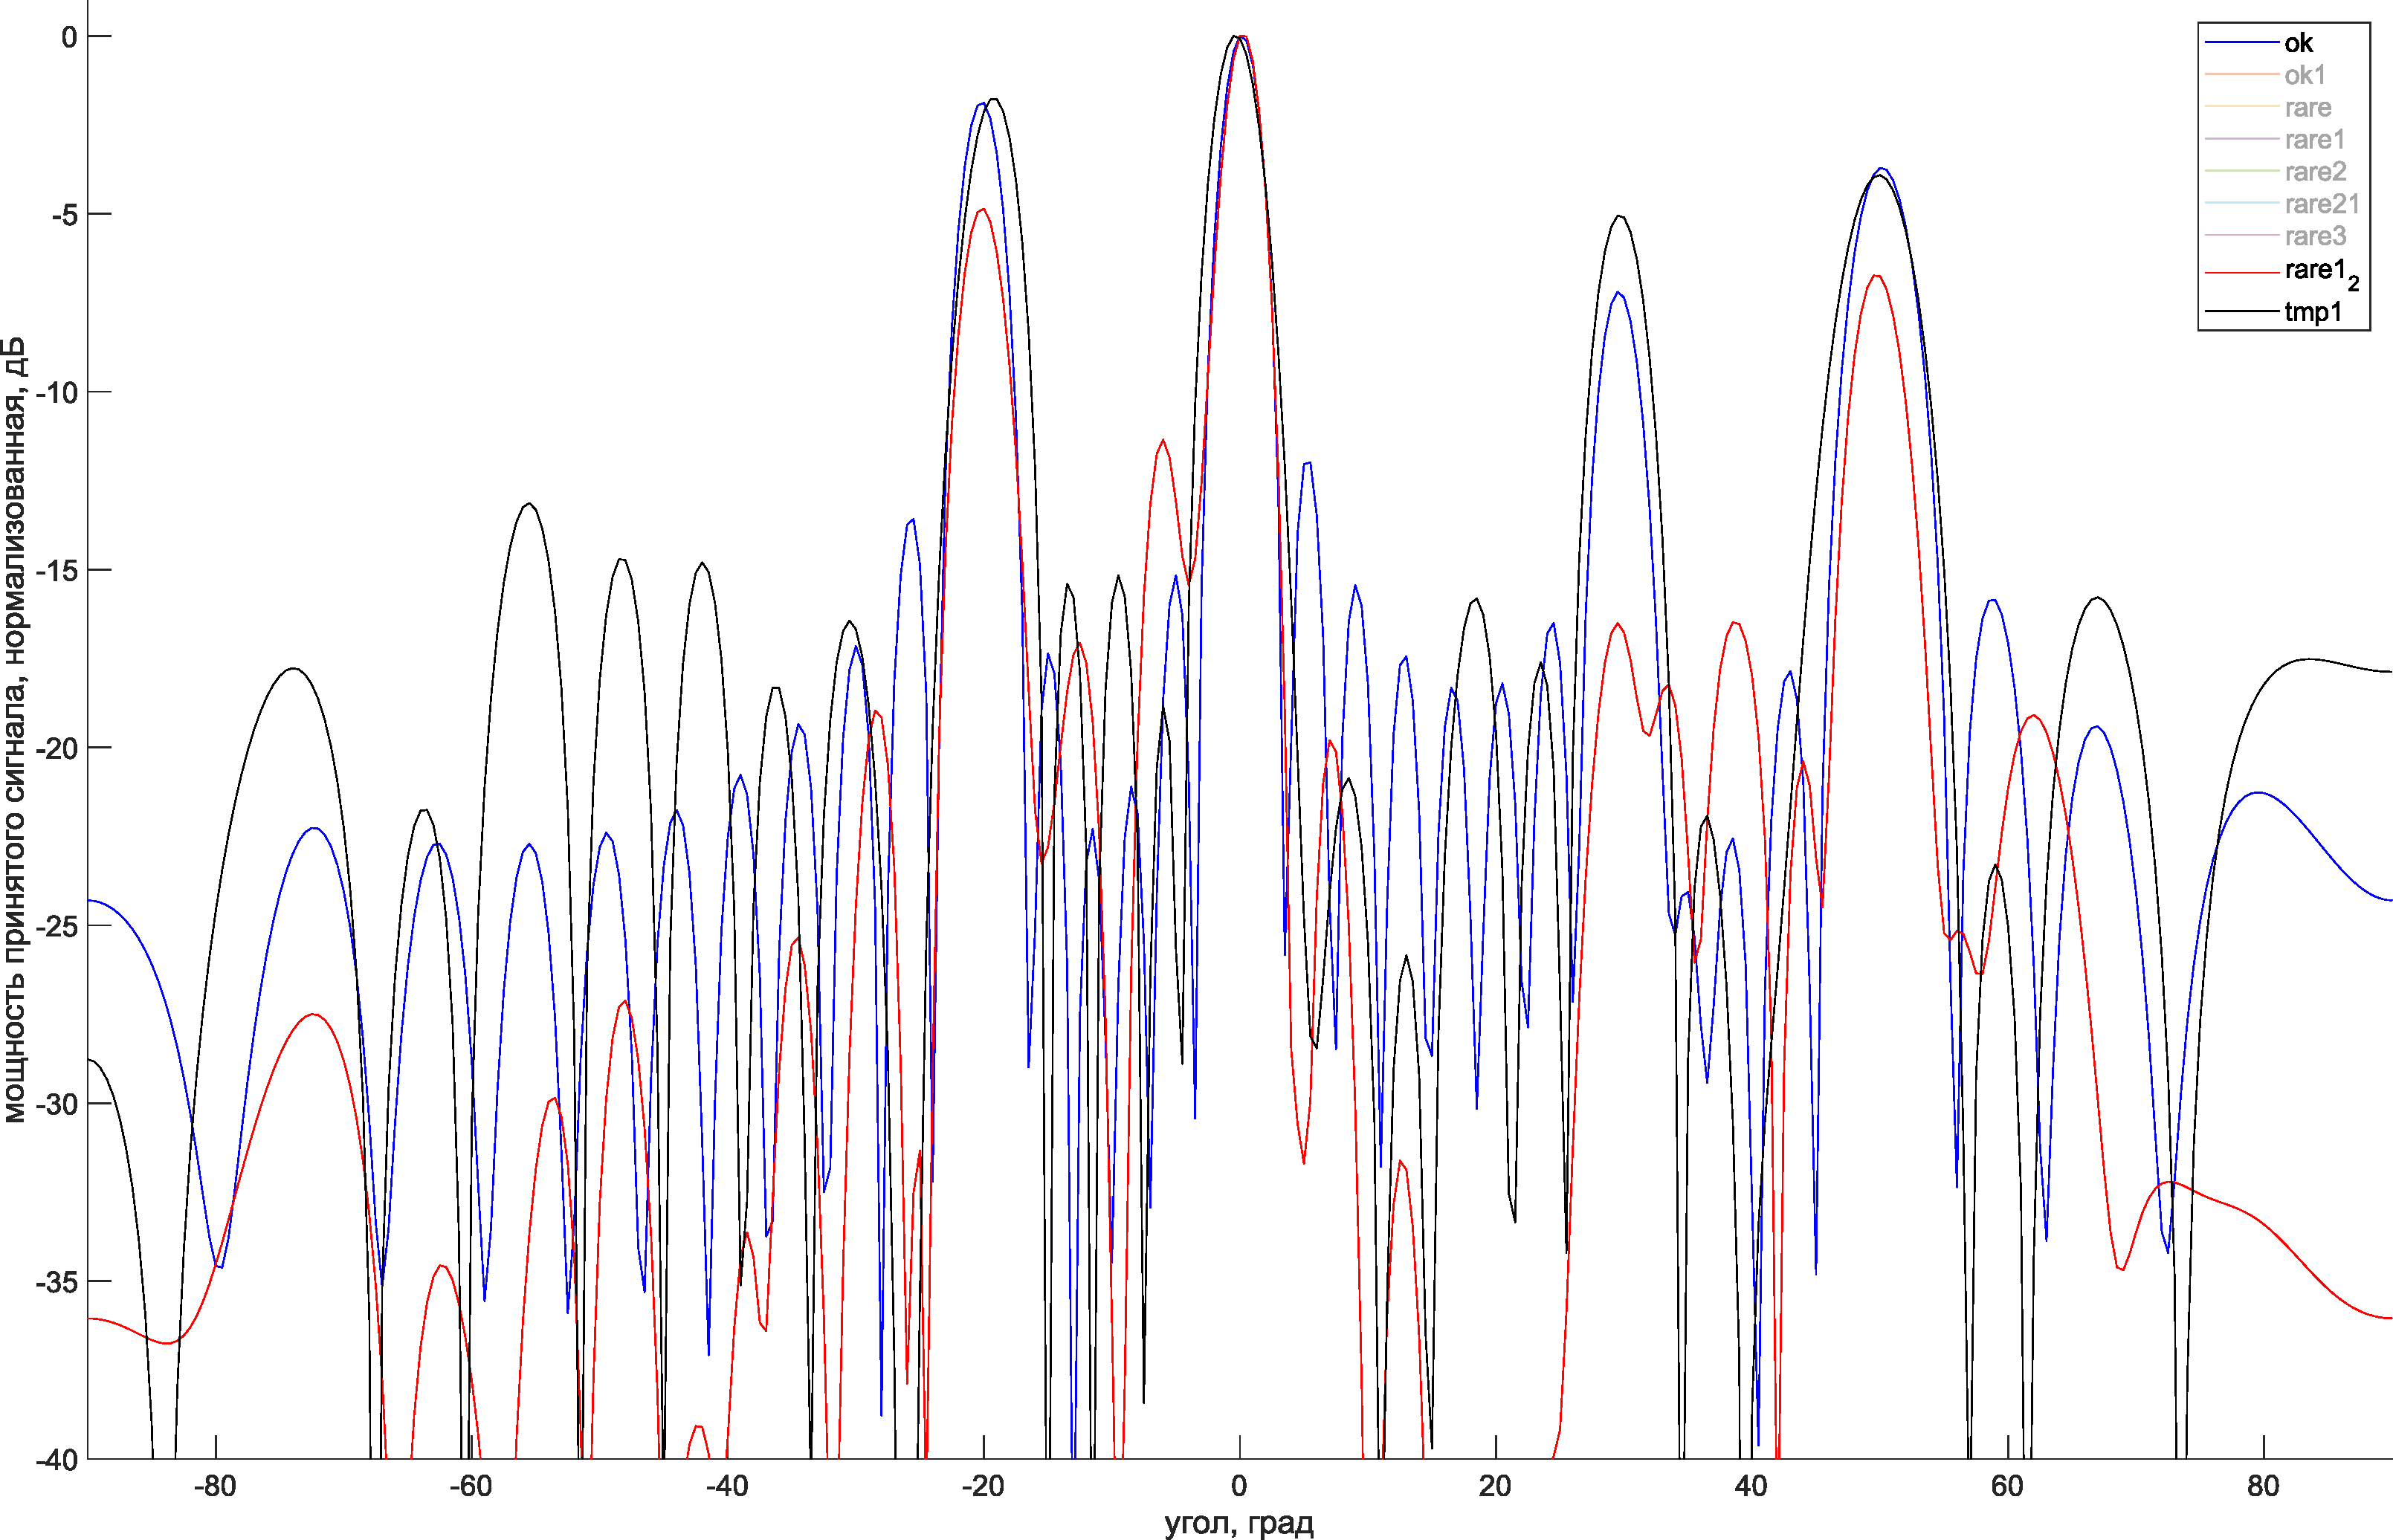
\includegraphics[width=0.8\textwidth,height=0.35\textheight,keepaspectratio]{iterative-array-demo}
    \caption{ Сравнение пространственного отклика для 3 решёток}%
    \label{fig:iterative-array-demo}
\end{figure}

Видно, что у разреженной решётки ниже уровень боковых лепестков, однако на большом количестве целей чётко 
<<вылезли>> дифракционные лепестки слева, в то время у АР синтезированной методом итераций, 
дифракционные лепестки имеют низкий уровень. 

В то же время обнаруживается проблема, связанная с тем, как в рассматриваемом методе объединяются данные 
от разных подрешёток -- сигнал, который на 4~дБ слабее других сигналов в рамках того же отсчёта по 
дальности, оказался подавлен на ещё 3~дБ. Можно избавиться от этой проблемы если использовать 
более интеллектуальные алгоритмы объединения результатов, однако это является 
темой дальнейших исследований и не рассматривается в данной работе.

\subsection{Заключение}

Данный подход использует возможности ЦАР по раздельной обработке данных из каждого канала. 
Он имеет следующие преимущества:

\begin{itemize}
    \item Алгоритм интуитивно понятен и легко воспроизводим
    \item Подавление боковых лепестков -- такой подход позволяет добиться меньшего уровня боковых лепестков чем массив с 
    равномерным расположением элементов и чем у разреженной решётки с расширяющимся к краям распределением
    \item Уменьшение количества -- в показанном примере в разреженной решетке на $33,33$\% элементов 
    меньше чем в эквидистантной
\end{itemize}

Однако он в то же время обладает следующими недостатками:

\begin{itemize}
    \item Сложность вычислений:
    \begin{itemize}
        \item неравномерное расположение элементов не позволяет использовать быстрое 
        преобразование Фурье для диаграммообразования
        \item так как одни и те же данные используются несколько раз для расчёта результатов для одного отсчёта по 
        дальности, то увеличивается время обработки одного отсчёта и усложняется 
        проектирование вычислительного конвейера
    \end{itemize}
    \item Подавление слабых сигналов - если в рамках одного отсчёта по дальности в области обзора находится несколько 
    источников с сильно отличающимся уровнями сигналов, то более слабые сигналы могут быть подавлены, и источник останется 
    незамеченной, что является серьезным недостатком в ряде применений, особенно в военной промышленности. Однако данный 
    недостаток может быть устранён, если применять иной, отличный от прямого перемножения, способ объединения результатов.
\end{itemize}

В целом, данный подход имеет перспективы, однако метод объединения результатов нуждается 
в усовершенствовании и проведении дальнейших исследований. 

